\documentclass[twoside]{book}

% Packages required by doxygen
\usepackage{fixltx2e}
\usepackage{calc}
\usepackage{doxygen}
\usepackage[export]{adjustbox} % also loads graphicx
\usepackage{graphicx}
\usepackage[utf8]{inputenc}
\usepackage{makeidx}
\usepackage{multicol}
\usepackage{multirow}
\PassOptionsToPackage{warn}{textcomp}
\usepackage{textcomp}
\usepackage[nointegrals]{wasysym}
\usepackage[table]{xcolor}

% Font selection
\usepackage[T1]{fontenc}
\usepackage[scaled=.90]{helvet}
\usepackage{courier}
\usepackage{amssymb}
\usepackage{sectsty}
\renewcommand{\familydefault}{\sfdefault}
\allsectionsfont{%
  \fontseries{bc}\selectfont%
  \color{darkgray}%
}
\renewcommand{\DoxyLabelFont}{%
  \fontseries{bc}\selectfont%
  \color{darkgray}%
}
\newcommand{\+}{\discretionary{\mbox{\scriptsize$\hookleftarrow$}}{}{}}

% Page & text layout
\usepackage{geometry}
\geometry{%
  a4paper,%
  top=2.5cm,%
  bottom=2.5cm,%
  left=2.5cm,%
  right=2.5cm%
}
\tolerance=750
\hfuzz=15pt
\hbadness=750
\setlength{\emergencystretch}{15pt}
\setlength{\parindent}{0cm}
\setlength{\parskip}{0.2cm}
\makeatletter
\renewcommand{\paragraph}{%
  \@startsection{paragraph}{4}{0ex}{-1.0ex}{1.0ex}{%
    \normalfont\normalsize\bfseries\SS@parafont%
  }%
}
\renewcommand{\subparagraph}{%
  \@startsection{subparagraph}{5}{0ex}{-1.0ex}{1.0ex}{%
    \normalfont\normalsize\bfseries\SS@subparafont%
  }%
}
\makeatother

% Headers & footers
\usepackage{fancyhdr}
\pagestyle{fancyplain}
\fancyhead[LE]{\fancyplain{}{\bfseries\thepage}}
\fancyhead[CE]{\fancyplain{}{}}
\fancyhead[RE]{\fancyplain{}{\bfseries\leftmark}}
\fancyhead[LO]{\fancyplain{}{\bfseries\rightmark}}
\fancyhead[CO]{\fancyplain{}{}}
\fancyhead[RO]{\fancyplain{}{\bfseries\thepage}}
\fancyfoot[LE]{\fancyplain{}{}}
\fancyfoot[CE]{\fancyplain{}{}}
\fancyfoot[RE]{\fancyplain{}{\bfseries\scriptsize Generated on Wed Dec 9 2015 18\+:53\+:37 for O\+S\+Net\+Shield by Doxygen }}
\fancyfoot[LO]{\fancyplain{}{\bfseries\scriptsize Generated on Wed Dec 9 2015 18\+:53\+:37 for O\+S\+Net\+Shield by Doxygen }}
\fancyfoot[CO]{\fancyplain{}{}}
\fancyfoot[RO]{\fancyplain{}{}}
\renewcommand{\footrulewidth}{0.4pt}
\renewcommand{\chaptermark}[1]{%
  \markboth{#1}{}%
}
\renewcommand{\sectionmark}[1]{%
  \markright{\thesection\ #1}%
}

% Indices & bibliography
\usepackage{natbib}
\usepackage[titles]{tocloft}
\setcounter{tocdepth}{3}
\setcounter{secnumdepth}{5}
\makeindex

% Hyperlinks (required, but should be loaded last)
\usepackage{ifpdf}
\ifpdf
  \usepackage[pdftex,pagebackref=true]{hyperref}
\else
  \usepackage[ps2pdf,pagebackref=true]{hyperref}
\fi
\hypersetup{%
  colorlinks=true,%
  linkcolor=blue,%
  citecolor=blue,%
  unicode%
}

% Custom commands
\newcommand{\clearemptydoublepage}{%
  \newpage{\pagestyle{empty}\cleardoublepage}%
}


%===== C O N T E N T S =====

\begin{document}

% Titlepage & ToC
\hypersetup{pageanchor=false,
             bookmarks=true,
             bookmarksnumbered=true,
             pdfencoding=unicode
            }
\pagenumbering{roman}
\begin{titlepage}
\vspace*{7cm}
\begin{center}%
{\Large O\+S\+Net\+Shield }\\
\vspace*{1cm}
{\large Generated by Doxygen 1.8.10}\\
\vspace*{0.5cm}
{\small Wed Dec 9 2015 18:53:37}\\
\end{center}
\end{titlepage}
\clearemptydoublepage
\tableofcontents
\clearemptydoublepage
\pagenumbering{arabic}
\hypersetup{pageanchor=true}

%--- Begin generated contents ---
\chapter{Hierarchical Index}
\section{Class Hierarchy}
This inheritance list is sorted roughly, but not completely, alphabetically\+:\begin{DoxyCompactList}
\item C\+Dialog\begin{DoxyCompactList}
\item \contentsline{section}{Basic\+\_\+window}{\pageref{class_basic__window}}{}
\item \contentsline{section}{T\+C\+P\+Form}{\pageref{class_t_c_p_form}}{}
\end{DoxyCompactList}
\item C\+Dialog\+Ex\begin{DoxyCompactList}
\item \contentsline{section}{Country\+Data\+Dialog}{\pageref{class_country_data_dialog}}{}
\end{DoxyCompactList}
\item \contentsline{section}{c\+Fw\+Access}{\pageref{classc_fw_access}}{}
\item \contentsline{section}{c\+I\+P}{\pageref{classc_i_p}}{}
\item \contentsline{section}{Country\+\_\+\+Data}{\pageref{class_country___data}}{}
\item \contentsline{section}{Country\+\_\+\+Data\+:\+:Value}{\pageref{struct_country___data_1_1_value}}{}
\end{DoxyCompactList}

\chapter{Class Index}
\section{Class List}
Here are the classes, structs, unions and interfaces with brief descriptions\+:\begin{DoxyCompactList}
\item\contentsline{section}{\hyperlink{class_basic__window}{Basic\+\_\+window} }{\pageref{class_basic__window}}{}
\item\contentsline{section}{\hyperlink{classc_fw_access}{c\+Fw\+Access} }{\pageref{classc_fw_access}}{}
\item\contentsline{section}{\hyperlink{classc_i_p}{c\+I\+P} }{\pageref{classc_i_p}}{}
\item\contentsline{section}{\hyperlink{class_country___data}{Country\+\_\+\+Data} }{\pageref{class_country___data}}{}
\item\contentsline{section}{\hyperlink{class_country_data_dialog}{Country\+Data\+Dialog} }{\pageref{class_country_data_dialog}}{}
\item\contentsline{section}{\hyperlink{class_t_c_p_form}{T\+C\+P\+Form} }{\pageref{class_t_c_p_form}}{}
\item\contentsline{section}{\hyperlink{struct_country___data_1_1_value}{Country\+\_\+\+Data\+::\+Value} }{\pageref{struct_country___data_1_1_value}}{}
\end{DoxyCompactList}

\chapter{Class Documentation}
\hypertarget{class_basic__window}{}\section{Basic\+\_\+window Class Reference}
\label{class_basic__window}\index{Basic\+\_\+window@{Basic\+\_\+window}}
Inheritance diagram for Basic\+\_\+window\+:\begin{figure}[H]
\begin{center}
\leavevmode
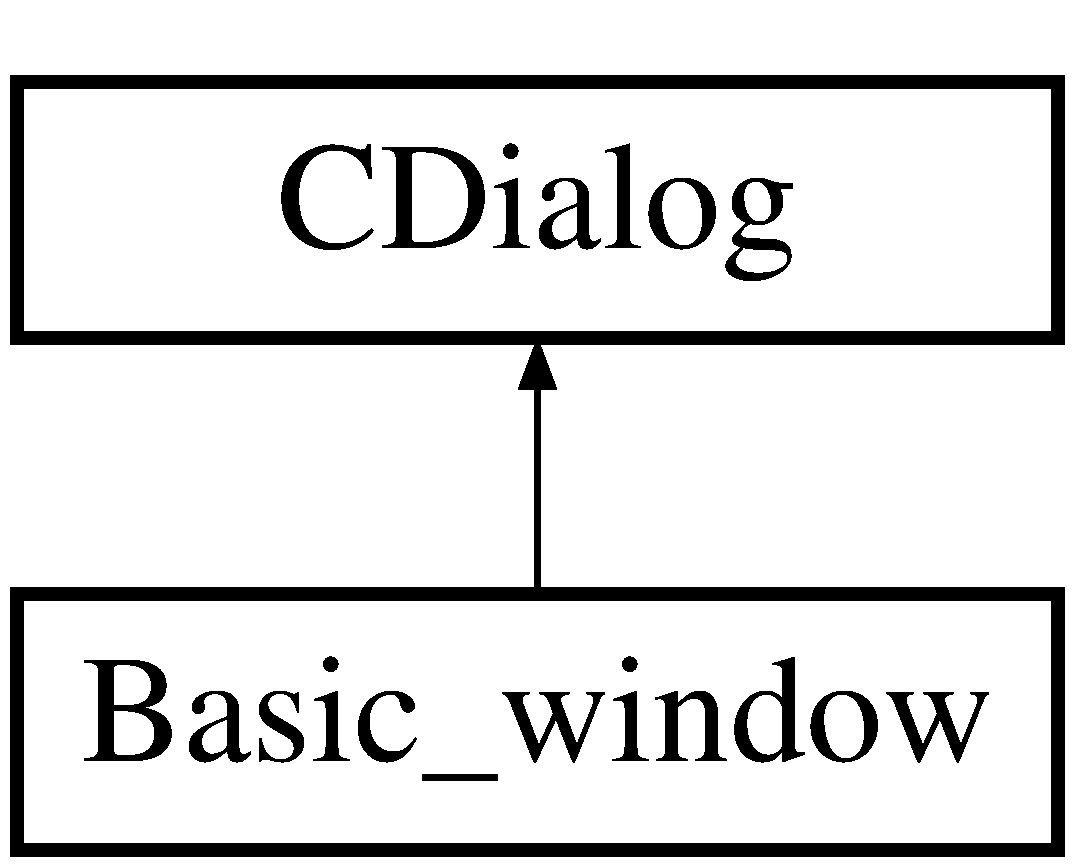
\includegraphics[height=2.000000cm]{class_basic__window}
\end{center}
\end{figure}
\subsection*{Public Types}
\begin{DoxyCompactItemize}
\item 
\hypertarget{class_basic__window_a2fb129e769a0ea51892cf6ed9fa7d988}{}enum \{ {\bfseries I\+D\+D} = I\+D\+D\+\_\+\+D\+I\+A\+L\+O\+G1
 \}\label{class_basic__window_a2fb129e769a0ea51892cf6ed9fa7d988}

\end{DoxyCompactItemize}
\subsection*{Public Member Functions}
\begin{DoxyCompactItemize}
\item 
\hypertarget{class_basic__window_ae4b70715ce8e59b6a6b94c4753e25fbb}{}{\bfseries Basic\+\_\+window} (\hyperlink{classc_fw_access}{c\+Fw\+Access} $\ast$p\+Fw\+Access\+In, C\+Wnd $\ast$p\+Parent=N\+U\+L\+L)\label{class_basic__window_ae4b70715ce8e59b6a6b94c4753e25fbb}

\item 
\hypertarget{class_basic__window_ab1979f288ca0de48bc348d8d37450467}{}afx\+\_\+msg void {\bfseries On\+Bn\+Clicked\+Block} ()\label{class_basic__window_ab1979f288ca0de48bc348d8d37450467}

\item 
\hypertarget{class_basic__window_a5fe3e664c30e5263f2df87fe60fc67ff}{}afx\+\_\+msg void {\bfseries On\+Bn\+Clicked\+Unblock} ()\label{class_basic__window_a5fe3e664c30e5263f2df87fe60fc67ff}

\item 
\hypertarget{class_basic__window_a500da75c42b6515cee14403cee29d4ff}{}afx\+\_\+msg void {\bfseries On\+En\+Change\+Edit1} ()\label{class_basic__window_a500da75c42b6515cee14403cee29d4ff}

\item 
\hypertarget{class_basic__window_a0565f352a1ecb13d6460288ac4f5af9e}{}afx\+\_\+msg void {\bfseries On\+En\+Change\+Edit2} ()\label{class_basic__window_a0565f352a1ecb13d6460288ac4f5af9e}

\item 
\hypertarget{class_basic__window_a362554cba60f4105745f10eedcf31005}{}afx\+\_\+msg void {\bfseries On\+Bn\+Clicked\+Button1} ()\label{class_basic__window_a362554cba60f4105745f10eedcf31005}

\item 
\hypertarget{class_basic__window_aa7e927a5635aee90f6732b6a2a286b31}{}afx\+\_\+msg void {\bfseries On\+Bn\+Clicked\+Button2} ()\label{class_basic__window_aa7e927a5635aee90f6732b6a2a286b31}

\item 
\hypertarget{class_basic__window_aee2e80f482c4ff694fe316a2e7af28e5}{}afx\+\_\+msg void {\bfseries On\+Bn\+Clicked\+Button3} ()\label{class_basic__window_aee2e80f482c4ff694fe316a2e7af28e5}

\end{DoxyCompactItemize}
\subsection*{Protected Member Functions}
\begin{DoxyCompactItemize}
\item 
\hypertarget{class_basic__window_a7ba1ea061979fb4fc4a08dcd07f11fb1}{}virtual void {\bfseries Do\+Data\+Exchange} (C\+Data\+Exchange $\ast$p\+D\+X)\label{class_basic__window_a7ba1ea061979fb4fc4a08dcd07f11fb1}

\end{DoxyCompactItemize}


The documentation for this class was generated from the following files\+:\begin{DoxyCompactItemize}
\item 
Basic\+\_\+window.\+h\item 
Basic\+\_\+window.\+cpp\end{DoxyCompactItemize}

\hypertarget{classc_fw_access}{}\section{c\+Fw\+Access Class Reference}
\label{classc_fw_access}\index{c\+Fw\+Access@{c\+Fw\+Access}}


{\ttfamily \#include $<$c\+Fw\+Access.\+h$>$}

\subsection*{Public Member Functions}
\begin{DoxyCompactItemize}
\item 
void \hyperlink{classc_fw_access_a08e2e69a2e96eed18f77c25819d467d4}{make\+Rule} (std\+::wstring \&s\+Name, std\+::wstring \&s\+Dscr, std\+::wstring \&s\+Addr, int n\+Action, N\+E\+T\+\_\+\+F\+W\+\_\+\+R\+U\+L\+E\+\_\+\+D\+I\+R\+E\+C\+T\+I\+O\+N\+\_\+ dir)
\item 
\hypertarget{classc_fw_access_a9eb66aa7d36c526b6617e69bead57915}{}void {\bfseries cleanup} (B\+S\+T\+R \&bstr\+Rule\+Name, B\+S\+T\+R \&bstr\+Rule\+Description, B\+S\+T\+R \&bstr\+Rule\+Group, B\+S\+T\+R \&bstr\+Rule\+Remote\+Adresses, B\+S\+T\+R \&bstr\+Val, I\+Net\+Fw\+Rule $\ast$p\+Fw\+Rule, I\+Net\+Fw\+Rules $\ast$p\+Fw\+Rules, I\+Net\+Fw\+Policy2 $\ast$p\+Net\+Fw\+Policy2, H\+R\+E\+S\+U\+L\+T \&hr\+Com\+Init)\label{classc_fw_access_a9eb66aa7d36c526b6617e69bead57915}

\item 
void \hyperlink{classc_fw_access_a26b6363cd83d1d54a318030e35552a6b}{Rule\+Unblocker} (B\+S\+T\+R \&bstr\+Rule\+Name, B\+S\+T\+R \&bstr\+Rule\+Description, B\+S\+T\+R \&bstr\+Rule\+Group, B\+S\+T\+R \&bstr\+Rule\+Remote\+Adresses, B\+S\+T\+R \&bstr\+Val, I\+Net\+Fw\+Rule $\ast$p\+Fw\+Rule, I\+Net\+Fw\+Rules $\ast$p\+Fw\+Rules, I\+Net\+Fw\+Policy2 $\ast$p\+Net\+Fw\+Policy2, H\+R\+E\+S\+U\+L\+T \&hr\+Com\+Init, H\+R\+E\+S\+U\+L\+T \&hr)
\item 
std\+::wstring \hyperlink{classc_fw_access_aefabb6d98360ce5ab95d14d2cc1bd896}{make\+Rule\+Name} ()
\item 
void \hyperlink{classc_fw_access_a6519f8ac419fcba5c037f514c2aea71b}{control\+Fw} ()
\item 
void \hyperlink{classc_fw_access_a8e969eb55aa4a9ca9af1710eb1bfb0ce}{control\+Fw\+G\+U\+I} (std\+::wstring \&s\+I\+P, int n\+Action)
\item 
bool \hyperlink{classc_fw_access_aa7b74e8ac58298c2582e3e2f5bd3265d}{is\+Wstring\+I\+P} (std\+::wstring \&str)
\end{DoxyCompactItemize}


\subsection{Detailed Description}
Class to manipulate Windows Firewall 

\subsection{Member Function Documentation}
\hypertarget{classc_fw_access_a6519f8ac419fcba5c037f514c2aea71b}{}\index{c\+Fw\+Access@{c\+Fw\+Access}!control\+Fw@{control\+Fw}}
\index{control\+Fw@{control\+Fw}!c\+Fw\+Access@{c\+Fw\+Access}}
\subsubsection[{control\+Fw()}]{\setlength{\rightskip}{0pt plus 5cm}void c\+Fw\+Access\+::control\+Fw (
\begin{DoxyParamCaption}
{}
\end{DoxyParamCaption}
)}\label{classc_fw_access_a6519f8ac419fcba5c037f514c2aea71b}
Manipulate the program using console \hypertarget{classc_fw_access_a8e969eb55aa4a9ca9af1710eb1bfb0ce}{}\index{c\+Fw\+Access@{c\+Fw\+Access}!control\+Fw\+G\+U\+I@{control\+Fw\+G\+U\+I}}
\index{control\+Fw\+G\+U\+I@{control\+Fw\+G\+U\+I}!c\+Fw\+Access@{c\+Fw\+Access}}
\subsubsection[{control\+Fw\+G\+U\+I(std\+::wstring \&s\+I\+P, int n\+Action)}]{\setlength{\rightskip}{0pt plus 5cm}void c\+Fw\+Access\+::control\+Fw\+G\+U\+I (
\begin{DoxyParamCaption}
\item[{std\+::wstring \&}]{s\+I\+P, }
\item[{int}]{n\+Action}
\end{DoxyParamCaption}
)}\label{classc_fw_access_a8e969eb55aa4a9ca9af1710eb1bfb0ce}
Manipulate the program using G\+U\+I \hypertarget{classc_fw_access_aa7b74e8ac58298c2582e3e2f5bd3265d}{}\index{c\+Fw\+Access@{c\+Fw\+Access}!is\+Wstring\+I\+P@{is\+Wstring\+I\+P}}
\index{is\+Wstring\+I\+P@{is\+Wstring\+I\+P}!c\+Fw\+Access@{c\+Fw\+Access}}
\subsubsection[{is\+Wstring\+I\+P(std\+::wstring \&str)}]{\setlength{\rightskip}{0pt plus 5cm}bool c\+Fw\+Access\+::is\+Wstring\+I\+P (
\begin{DoxyParamCaption}
\item[{std\+::wstring \&}]{str}
\end{DoxyParamCaption}
)}\label{classc_fw_access_aa7b74e8ac58298c2582e3e2f5bd3265d}
Determine if the wstring can be interpreted as an I\+P address \hypertarget{classc_fw_access_a08e2e69a2e96eed18f77c25819d467d4}{}\index{c\+Fw\+Access@{c\+Fw\+Access}!make\+Rule@{make\+Rule}}
\index{make\+Rule@{make\+Rule}!c\+Fw\+Access@{c\+Fw\+Access}}
\subsubsection[{make\+Rule(std\+::wstring \&s\+Name, std\+::wstring \&s\+Dscr, std\+::wstring \&s\+Addr, int n\+Action, N\+E\+T\+\_\+\+F\+W\+\_\+\+R\+U\+L\+E\+\_\+\+D\+I\+R\+E\+C\+T\+I\+O\+N\+\_\+ dir)}]{\setlength{\rightskip}{0pt plus 5cm}void c\+Fw\+Access\+::make\+Rule (
\begin{DoxyParamCaption}
\item[{std\+::wstring \&}]{s\+Name, }
\item[{std\+::wstring \&}]{s\+Dscr, }
\item[{std\+::wstring \&}]{s\+Addr, }
\item[{int}]{n\+Action, }
\item[{N\+E\+T\+\_\+\+F\+W\+\_\+\+R\+U\+L\+E\+\_\+\+D\+I\+R\+E\+C\+T\+I\+O\+N\+\_\+}]{dir}
\end{DoxyParamCaption}
)}\label{classc_fw_access_a08e2e69a2e96eed18f77c25819d467d4}
Adding (n\+Action = 1) and removing rules (n\+Action = 2) Filling v\+Fw\+Added\+Rules with previously added rules (n\+Action = 0) (used for proper naming) \hypertarget{classc_fw_access_aefabb6d98360ce5ab95d14d2cc1bd896}{}\index{c\+Fw\+Access@{c\+Fw\+Access}!make\+Rule\+Name@{make\+Rule\+Name}}
\index{make\+Rule\+Name@{make\+Rule\+Name}!c\+Fw\+Access@{c\+Fw\+Access}}
\subsubsection[{make\+Rule\+Name()}]{\setlength{\rightskip}{0pt plus 5cm}std\+::wstring c\+Fw\+Access\+::make\+Rule\+Name (
\begin{DoxyParamCaption}
{}
\end{DoxyParamCaption}
)}\label{classc_fw_access_aefabb6d98360ce5ab95d14d2cc1bd896}
The method creates a name for a new rule Although it\textquotesingle{}s possible to create rules with same names, the names must differ for proper rule deleting The naming is based on wstrings in v\+Fw\+Added\+Rules from \hyperlink{classc_fw_access}{c\+Fw\+Access} class, which contains the names of the previously added rules The name of the new rule looks like \char`\"{}\+O\+S\+Net\+Shield\char`\"{} + the smallest available number std\+::string make\+Rule\+Name(std\+::vector$<$std\+::wstring$>$ \&v\+Fw\+Added\+Rules); \hypertarget{classc_fw_access_a26b6363cd83d1d54a318030e35552a6b}{}\index{c\+Fw\+Access@{c\+Fw\+Access}!Rule\+Unblocker@{Rule\+Unblocker}}
\index{Rule\+Unblocker@{Rule\+Unblocker}!c\+Fw\+Access@{c\+Fw\+Access}}
\subsubsection[{Rule\+Unblocker(\+B\+S\+T\+R \&bstr\+Rule\+Name, B\+S\+T\+R \&bstr\+Rule\+Description, B\+S\+T\+R \&bstr\+Rule\+Group, B\+S\+T\+R \&bstr\+Rule\+Remote\+Adresses, B\+S\+T\+R \&bstr\+Val, I\+Net\+Fw\+Rule $\ast$p\+Fw\+Rule, I\+Net\+Fw\+Rules $\ast$p\+Fw\+Rules, I\+Net\+Fw\+Policy2 $\ast$p\+Net\+Fw\+Policy2, H\+R\+E\+S\+U\+L\+T \&hr\+Com\+Init, H\+R\+E\+S\+U\+L\+T \&hr)}]{\setlength{\rightskip}{0pt plus 5cm}void c\+Fw\+Access\+::\+Rule\+Unblocker (
\begin{DoxyParamCaption}
\item[{B\+S\+T\+R \&}]{bstr\+Rule\+Name, }
\item[{B\+S\+T\+R \&}]{bstr\+Rule\+Description, }
\item[{B\+S\+T\+R \&}]{bstr\+Rule\+Group, }
\item[{B\+S\+T\+R \&}]{bstr\+Rule\+Remote\+Adresses, }
\item[{B\+S\+T\+R \&}]{bstr\+Val, }
\item[{I\+Net\+Fw\+Rule $\ast$}]{p\+Fw\+Rule, }
\item[{I\+Net\+Fw\+Rules $\ast$}]{p\+Fw\+Rules, }
\item[{I\+Net\+Fw\+Policy2 $\ast$}]{p\+Net\+Fw\+Policy2, }
\item[{H\+R\+E\+S\+U\+L\+T \&}]{hr\+Com\+Init, }
\item[{H\+R\+E\+S\+U\+L\+T \&}]{hr}
\end{DoxyParamCaption}
)}\label{classc_fw_access_a26b6363cd83d1d54a318030e35552a6b}
Method allows to avoid many repetitions in make\+Rule method In general, it removes a single rule (for both inbound and outbound connection) 

The documentation for this class was generated from the following files\+:\begin{DoxyCompactItemize}
\item 
c\+Fw\+Access.\+h\item 
c\+Fw\+Access.\+cpp\end{DoxyCompactItemize}

\hypertarget{classc_i_p}{}\section{c\+I\+P Class Reference}
\label{classc_i_p}\index{c\+I\+P@{c\+I\+P}}


{\ttfamily \#include $<$c\+Fw\+Access.\+h$>$}

\subsection*{Public Member Functions}
\begin{DoxyCompactItemize}
\item 
\hypertarget{classc_i_p_ae9d9e90ce86313975ada70a76439d867}{}{\bfseries c\+I\+P} (std\+::wstring \&str)\label{classc_i_p_ae9d9e90ce86313975ada70a76439d867}

\item 
\hypertarget{classc_i_p_aca751ad714dfdf3d2d68978cdd2f991c}{}std\+::wstring {\bfseries get\+Address} ()\label{classc_i_p_aca751ad714dfdf3d2d68978cdd2f991c}

\item 
void \hyperlink{classc_i_p_a8c02fa1e70a46745e18d8305b3f6e80c}{operator++} ()
\item 
void \hyperlink{classc_i_p_a7941c75ef13e4df9abb263f3af12d629}{operator-\/-\/} ()
\end{DoxyCompactItemize}


\subsection{Detailed Description}
Class to ease the work with I\+Ps Allows to move to the previous or next I\+P easily 

\subsection{Member Function Documentation}
\hypertarget{classc_i_p_a8c02fa1e70a46745e18d8305b3f6e80c}{}\index{c\+I\+P@{c\+I\+P}!operator++@{operator++}}
\index{operator++@{operator++}!c\+I\+P@{c\+I\+P}}
\subsubsection[{operator++()}]{\setlength{\rightskip}{0pt plus 5cm}void c\+I\+P\+::operator++ (
\begin{DoxyParamCaption}
{}
\end{DoxyParamCaption}
)}\label{classc_i_p_a8c02fa1e70a46745e18d8305b3f6e80c}
The next I\+P \hypertarget{classc_i_p_a7941c75ef13e4df9abb263f3af12d629}{}\index{c\+I\+P@{c\+I\+P}!operator-\/-\/@{operator-\/-\/}}
\index{operator-\/-\/@{operator-\/-\/}!c\+I\+P@{c\+I\+P}}
\subsubsection[{operator-\/-\/()}]{\setlength{\rightskip}{0pt plus 5cm}void c\+I\+P\+::operator-\/-\/ (
\begin{DoxyParamCaption}
{}
\end{DoxyParamCaption}
)}\label{classc_i_p_a7941c75ef13e4df9abb263f3af12d629}
The previous I\+P 

The documentation for this class was generated from the following files\+:\begin{DoxyCompactItemize}
\item 
c\+Fw\+Access.\+h\item 
c\+Fw\+Access.\+cpp\end{DoxyCompactItemize}

\hypertarget{class_country___data}{}\section{Country\+\_\+\+Data Class Reference}
\label{class_country___data}\index{Country\+\_\+\+Data@{Country\+\_\+\+Data}}
\subsection*{Classes}
\begin{DoxyCompactItemize}
\item 
struct \hyperlink{struct_country___data_1_1_value}{Value}
\end{DoxyCompactItemize}
\subsection*{Public Member Functions}
\begin{DoxyCompactItemize}
\item 
\hypertarget{class_country___data_ad8cd8e685a11d2c3e15586765f3e82b0}{}std\+::string {\bfseries Update\+D\+B} (C\+String s)\label{class_country___data_ad8cd8e685a11d2c3e15586765f3e82b0}

\item 
\hypertarget{class_country___data_aeb6c9e9291cf5330e8a34b57834db549}{}void {\bfseries print} ()\label{class_country___data_aeb6c9e9291cf5330e8a34b57834db549}

\end{DoxyCompactItemize}
\subsection*{Public Attributes}
\begin{DoxyCompactItemize}
\item 
\hypertarget{class_country___data_a84a1f119a29d9cc565f97f209cf73c03}{}std\+::vector$<$ \hyperlink{struct_country___data_1_1_value}{Value} $>$ {\bfseries Base}\label{class_country___data_a84a1f119a29d9cc565f97f209cf73c03}

\item 
\hypertarget{class_country___data_a2d51faac28584061816d53dfbbeabb55}{}int {\bfseries amount}\label{class_country___data_a2d51faac28584061816d53dfbbeabb55}

\end{DoxyCompactItemize}


The documentation for this class was generated from the following files\+:\begin{DoxyCompactItemize}
\item 
Country\+\_\+\+Data.\+h\item 
Country\+\_\+\+Data.\+cpp\end{DoxyCompactItemize}

\hypertarget{class_country_data_dialog}{}\section{Country\+Data\+Dialog Class Reference}
\label{class_country_data_dialog}\index{Country\+Data\+Dialog@{Country\+Data\+Dialog}}
Inheritance diagram for Country\+Data\+Dialog\+:\begin{figure}[H]
\begin{center}
\leavevmode
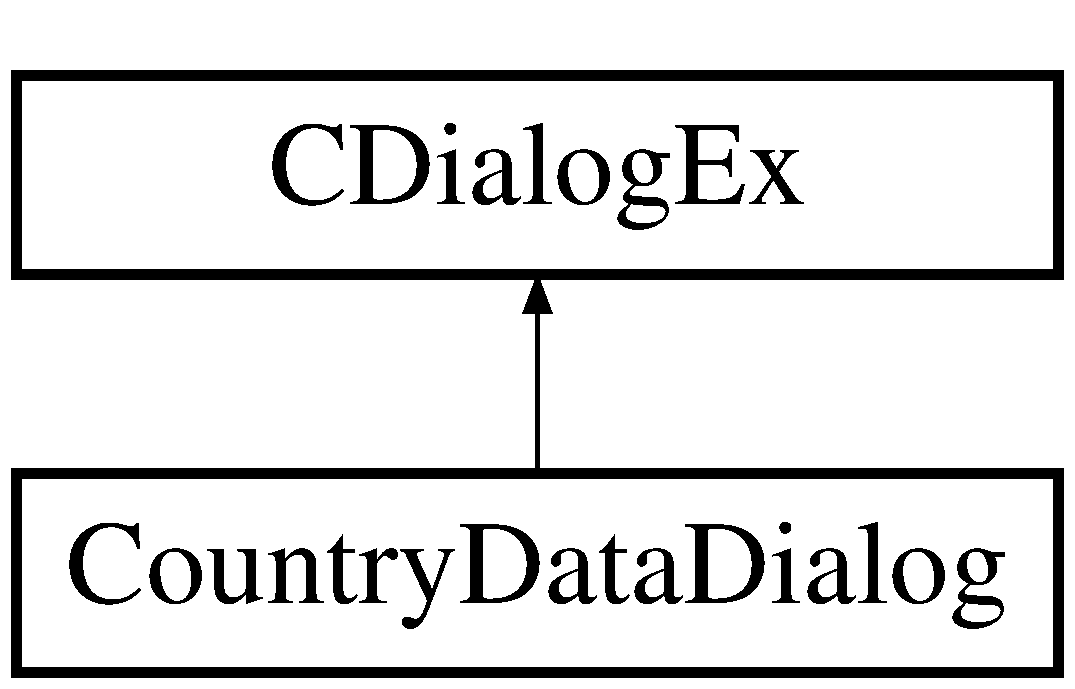
\includegraphics[height=2.000000cm]{class_country_data_dialog}
\end{center}
\end{figure}
\subsection*{Public Types}
\begin{DoxyCompactItemize}
\item 
\hypertarget{class_country_data_dialog_a9a6d29667d309efe43cc761537a1e0ac}{}enum \{ {\bfseries I\+D\+D} = I\+D\+D\+\_\+\+D\+I\+A\+L\+O\+G3
 \}\label{class_country_data_dialog_a9a6d29667d309efe43cc761537a1e0ac}

\end{DoxyCompactItemize}
\subsection*{Public Member Functions}
\begin{DoxyCompactItemize}
\item 
\hypertarget{class_country_data_dialog_a3a7e2efa6917b2261efb3ba84f7099a2}{}{\bfseries Country\+Data\+Dialog} (\hyperlink{classc_fw_access}{c\+Fw\+Access} $\ast$p\+Fw\+Access\+In, C\+Wnd $\ast$p\+Parent=N\+U\+L\+L)\label{class_country_data_dialog_a3a7e2efa6917b2261efb3ba84f7099a2}

\item 
\hypertarget{class_country_data_dialog_aa25b8873198744578c6a68b649e8a314}{}afx\+\_\+msg void {\bfseries On\+Bn\+Clicked\+Button1} ()\label{class_country_data_dialog_aa25b8873198744578c6a68b649e8a314}

\item 
\hypertarget{class_country_data_dialog_afaa4b2211333cdb0f0a9bf881c070c75}{}afx\+\_\+msg void {\bfseries On\+Bn\+Clicked\+Button2} ()\label{class_country_data_dialog_afaa4b2211333cdb0f0a9bf881c070c75}

\item 
\hypertarget{class_country_data_dialog_a64a2d07e544eca3f778871916bc06065}{}afx\+\_\+msg void {\bfseries On\+Bn\+Clicked\+Button3} ()\label{class_country_data_dialog_a64a2d07e544eca3f778871916bc06065}

\item 
\hypertarget{class_country_data_dialog_ab671b7b0d1169a75f2f3a45387dd6809}{}afx\+\_\+msg void {\bfseries On\+Cbn\+Selchange\+Combo1} ()\label{class_country_data_dialog_ab671b7b0d1169a75f2f3a45387dd6809}

\end{DoxyCompactItemize}
\subsection*{Public Attributes}
\begin{DoxyCompactItemize}
\item 
\hypertarget{class_country_data_dialog_ab031288bac4638e8d1d1965f61b4fcf9}{}\hyperlink{class_country___data}{Country\+\_\+\+Data} {\bfseries Data\+Base}\label{class_country_data_dialog_ab031288bac4638e8d1d1965f61b4fcf9}

\item 
\hypertarget{class_country_data_dialog_a86e512c68fc0efd0f9220e97ecb28a8b}{}C\+Combo\+Box {\bfseries Combo}\label{class_country_data_dialog_a86e512c68fc0efd0f9220e97ecb28a8b}

\end{DoxyCompactItemize}
\subsection*{Protected Member Functions}
\begin{DoxyCompactItemize}
\item 
\hypertarget{class_country_data_dialog_a0a8b5d4168cc358ebc0762f7e07bda6a}{}virtual void {\bfseries Do\+Data\+Exchange} (C\+Data\+Exchange $\ast$p\+D\+X)\label{class_country_data_dialog_a0a8b5d4168cc358ebc0762f7e07bda6a}

\end{DoxyCompactItemize}


The documentation for this class was generated from the following files\+:\begin{DoxyCompactItemize}
\item 
Country\+Data\+Dialog.\+h\item 
Country\+Data\+Dialog.\+cpp\end{DoxyCompactItemize}

\hypertarget{class_t_c_p_form}{}\section{T\+C\+P\+Form Class Reference}
\label{class_t_c_p_form}\index{T\+C\+P\+Form@{T\+C\+P\+Form}}
Inheritance diagram for T\+C\+P\+Form\+:\begin{figure}[H]
\begin{center}
\leavevmode
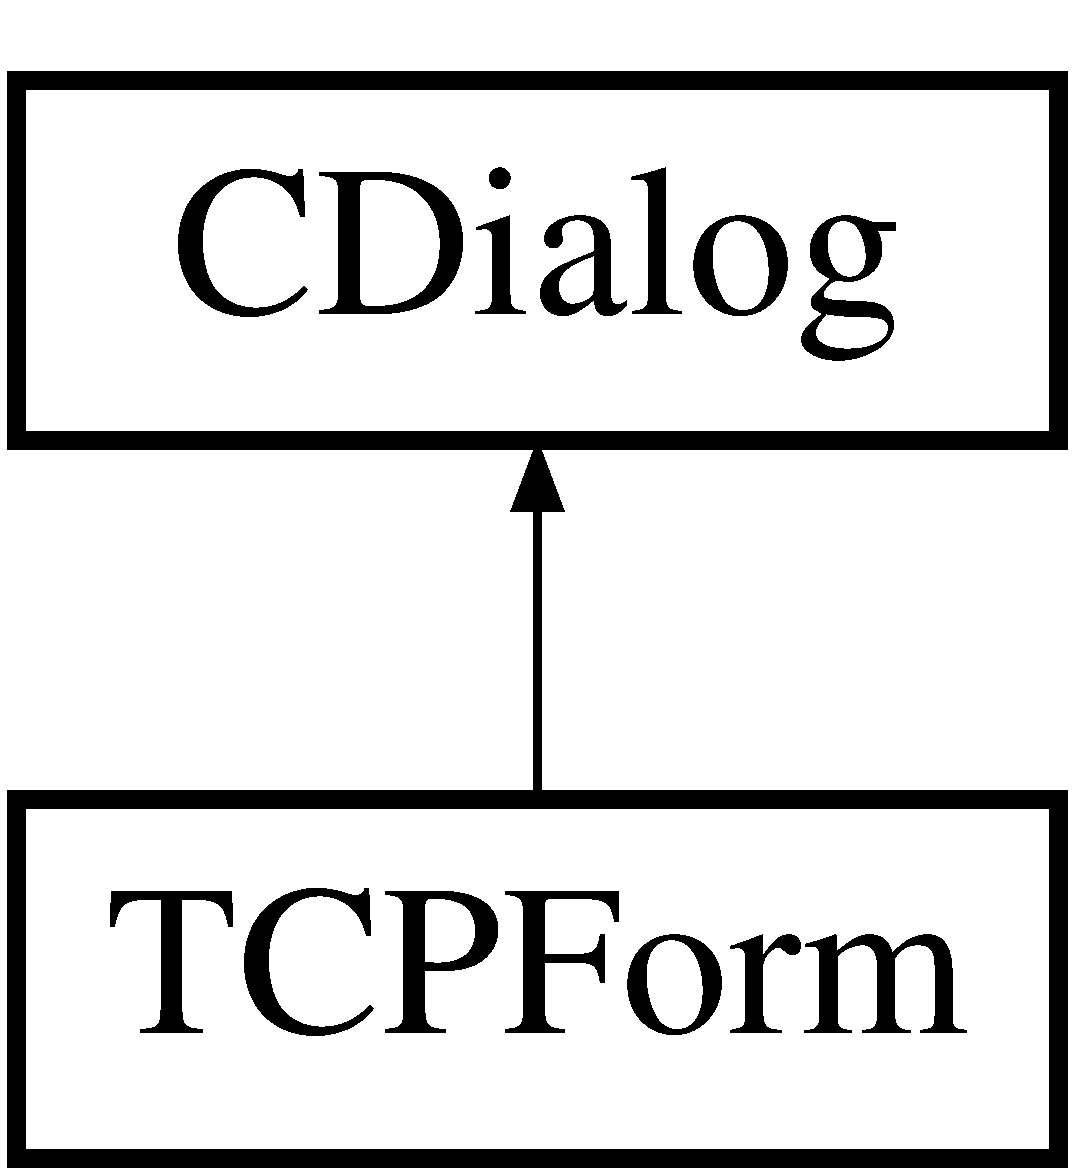
\includegraphics[height=2.000000cm]{class_t_c_p_form}
\end{center}
\end{figure}
\subsection*{Public Types}
\begin{DoxyCompactItemize}
\item 
\hypertarget{class_t_c_p_form_afb567f7a48a09bbff66797881a034c53}{}enum \{ {\bfseries I\+D\+D} = I\+D\+D\+\_\+\+D\+I\+A\+L\+O\+G2
 \}\label{class_t_c_p_form_afb567f7a48a09bbff66797881a034c53}

\end{DoxyCompactItemize}
\subsection*{Public Member Functions}
\begin{DoxyCompactItemize}
\item 
\hypertarget{class_t_c_p_form_a83410ff301d7a5068f040526e273128b}{}{\bfseries T\+C\+P\+Form} (C\+Wnd $\ast$p\+Parent=N\+U\+L\+L)\label{class_t_c_p_form_a83410ff301d7a5068f040526e273128b}

\item 
\hypertarget{class_t_c_p_form_aabec98179786dec8b2d157ffce755154}{}void {\bfseries Hide\+Label} ()\label{class_t_c_p_form_aabec98179786dec8b2d157ffce755154}

\item 
\hypertarget{class_t_c_p_form_ae5da34b74e9523384d961c4afe804616}{}afx\+\_\+msg void {\bfseries On\+Bn\+Clicked\+Ok} ()\label{class_t_c_p_form_ae5da34b74e9523384d961c4afe804616}

\item 
\hypertarget{class_t_c_p_form_af7bed7f1074e18ccc8b8f833028080a3}{}afx\+\_\+msg void {\bfseries On\+Bn\+Clicked\+Button1} ()\label{class_t_c_p_form_af7bed7f1074e18ccc8b8f833028080a3}

\end{DoxyCompactItemize}
\subsection*{Protected Member Functions}
\begin{DoxyCompactItemize}
\item 
\hypertarget{class_t_c_p_form_a904b920b81304813238dfe147cdb00c5}{}virtual void {\bfseries Do\+Data\+Exchange} (C\+Data\+Exchange $\ast$p\+D\+X)\label{class_t_c_p_form_a904b920b81304813238dfe147cdb00c5}

\end{DoxyCompactItemize}


The documentation for this class was generated from the following files\+:\begin{DoxyCompactItemize}
\item 
T\+C\+P\+Form.\+h\item 
T\+C\+P\+Form.\+cpp\end{DoxyCompactItemize}

\hypertarget{struct_country___data_1_1_value}{}\section{Country\+\_\+\+Data\+:\+:Value Struct Reference}
\label{struct_country___data_1_1_value}\index{Country\+\_\+\+Data\+::\+Value@{Country\+\_\+\+Data\+::\+Value}}
\subsection*{Public Attributes}
\begin{DoxyCompactItemize}
\item 
\hypertarget{struct_country___data_1_1_value_aca0781b09da67f07ec817432b0be82fc}{}std\+::string {\bfseries Short\+Name}\label{struct_country___data_1_1_value_aca0781b09da67f07ec817432b0be82fc}

\item 
\hypertarget{struct_country___data_1_1_value_a39b3463caef9a86b5848ef18c6df837d}{}std\+::string {\bfseries Long\+Name}\label{struct_country___data_1_1_value_a39b3463caef9a86b5848ef18c6df837d}

\item 
\hypertarget{struct_country___data_1_1_value_a10fc8d2a53fd927c8ca62ba5058b38ab}{}in\+\_\+addr {\bfseries from}\label{struct_country___data_1_1_value_a10fc8d2a53fd927c8ca62ba5058b38ab}

\item 
\hypertarget{struct_country___data_1_1_value_a2e6b769c0e288a62ebc8bf0ae9d9e23c}{}in\+\_\+addr {\bfseries to}\label{struct_country___data_1_1_value_a2e6b769c0e288a62ebc8bf0ae9d9e23c}

\end{DoxyCompactItemize}


The documentation for this struct was generated from the following file\+:\begin{DoxyCompactItemize}
\item 
Country\+\_\+\+Data.\+h\end{DoxyCompactItemize}

%--- End generated contents ---

% Index
\backmatter
\newpage
\phantomsection
\clearemptydoublepage
\addcontentsline{toc}{chapter}{Index}
\printindex

\end{document}
